\section*{Anexos}
\addcontentsline{toc}{section}{Anexos}

\subsection*{Árbol de problemas}
\addcontentsline{toc}{subsection}{Árbol de problemas}

\textbf{Problema Principal:}

\vspace{0.3cm}
Detección tardía del riesgo de shock hemorrágico en pacientes sometidos a cirugía mayor no cardiaca postoperatoria

\vspace{0.5cm}
\textbf{Causas:}

\begin{itemize}
    \item \textbf{Causa 1: Dependencia exclusiva de la experiencia médica}
    \begin{itemize}
        \item Sub-causa 1: Variabilidad en la interpretación clínica
        \begin{itemize}
            \item Sub-sub-causa 1: Diferencias en criterios diagnósticos entre profesionales
            \item Sub-sub-causa 2: Falta de protocolos estandarizados de evaluación
        \end{itemize}
        \item Sub-causa 2: Sesgos cognitivos en la toma de decisiones clínicas
        \item Sub-causa 3: Limitaciones humanas en el monitoreo continuo
        \begin{itemize}
            \item Sub-sub-causa 1: Fatiga del personal médico durante procedimientos prolongados
            \item Sub-sub-causa 2: Dificultad para detectar cambios sutiles en signos vitales
            \item Sub-sub-causa 3: Sobrecarga de información durante situaciones críticas
        \end{itemize}
    \end{itemize}
    
    \item \textbf{Causa 2: Protocolos clínicos no actualizados}
    \begin{itemize}
        \item Sub-causa 1: Enfoque reactivo en lugar de predictivo
        \item Sub-causa 2: Criterios diagnósticos basados en manifestaciones tardías
        \item Sub-causa 3: No consideración de factores de riesgo individuales
    \end{itemize}
    
    \item \textbf{Causa 3: Escasa personalización según características del paciente}
    \begin{itemize}
        \item Sub-causa 1: Ignorancia de comorbilidades específicas
        \item Sub-causa 2: Falta de adaptación a características demográficas
    \end{itemize}
\end{itemize}

\vspace{0.5cm}
\textbf{Efectos:}

\begin{itemize}
    \item \textbf{Efecto 1: Aumento de la mortalidad postoperatoria}
    \begin{itemize}
        \item Sub-efecto 1: Muertes por hemorragia no controlada
        \item Sub-efecto 2: Daño irreversible a órganos por hipoperfusión prolongada
        \item Sub-efecto 3: Mayor riesgo de infecciones postoperatorias
        \item Sub-efecto 4: Falla multiorgánica por manejo tardío
    \end{itemize}
    
    \item \textbf{Efecto 2: Mayor necesidad de transfusiones sanguíneas}
    \begin{itemize}
        \item Sub-efecto 1: Uso ineficiente de recursos sanguíneos
        \begin{itemize}
            \item Sub-sub-efecto 1: Transfusiones reactivas en lugar de preventivas
            \item Sub-sub-efecto 2: Escasez de hemoderivados en momentos críticos
            \item Sub-sub-efecto 3: Mayor riesgo de reacciones adversas
        \end{itemize}
        \item Sub-efecto 2: Complicaciones asociadas a transfusiones
        \begin{itemize}
            \item Sub-sub-efecto 1: Sobrecarga circulatoria
            \item Sub-sub-efecto 2: Reacciones inmunológicas
            \item Sub-sub-efecto 3: Mayor riesgo de infecciones
        \end{itemize}
    \end{itemize}
    
    \item \textbf{Efecto 3: Incremento de complicaciones postoperatorias}
    \begin{itemize}
        \item Sub-efecto 1: Daño orgánico por hipoperfusión prolongada
        \begin{itemize}
            \item Sub-sub-efecto 1: Insuficiencia renal aguda
            \item Sub-sub-efecto 2: Daño cerebral por hipoxia
            \item Sub-sub-efecto 3: Necrosis intestinal
        \end{itemize}
        \item Sub-efecto 2: Prolongación de la recuperación
        \begin{itemize}
            \item Sub-sub-efecto 1: Necesidad de cirugías adicionales correctivas
            \item Sub-sub-efecto 2: Rehabilitación más compleja y prolongada
        \end{itemize}
    \end{itemize}
    
    \item \textbf{Efecto 4: Impacto económico y en recursos hospitalarios}
    \begin{itemize}
        \item Sub-efecto 1: Aumento de los costos médicos
        \begin{itemize}
            \item Sub-sub-efecto 1: Mayor duración de la estancia hospitalaria
            \item Sub-sub-efecto 2: Uso excesivo de recursos críticos (UCI, sangre, medicamentos)
            \item Sub-sub-efecto 3: Costos adicionales por manejo de complicaciones
        \end{itemize}
        \item Sub-efecto 2: Saturación de recursos hospitalarios
    \end{itemize}
\end{itemize}

\newpage

\subsection*{Cronograma}
\addcontentsline{toc}{subsection}{Cronograma}

\begin{figure}[H]
\centering
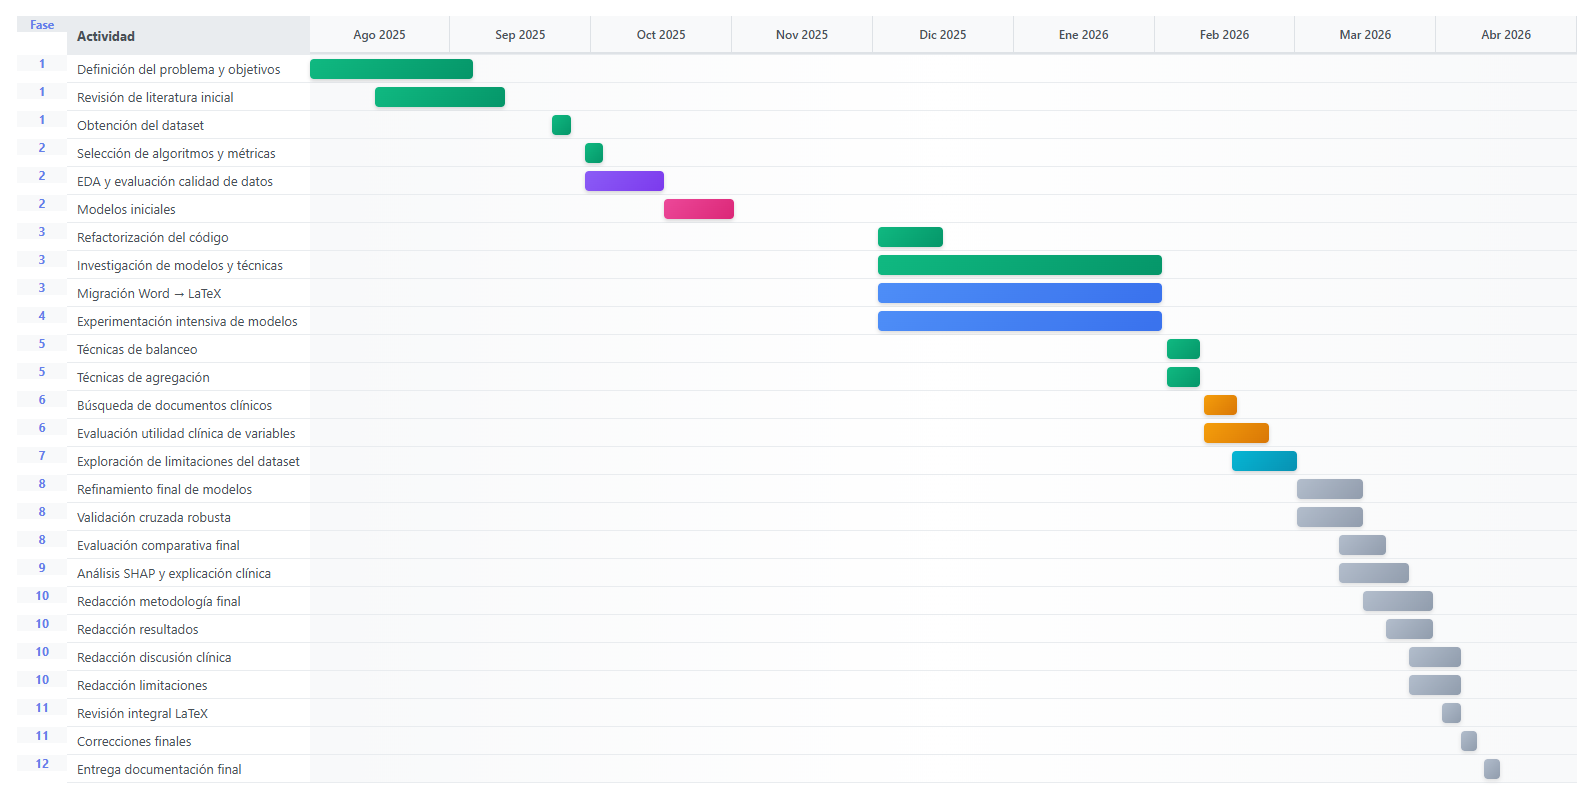
\includegraphics[width=\textwidth]{images/image025.png}
\caption{Cronograma detallado del Proyecto de Grado en Inteligencia Artificial, elaborado mediante TeamGantt}
\end{figure}

\subsection*{Análisis de Participación}
\addcontentsline{toc}{subsection}{Análisis de Participación}

\begin{itemize}
    \item Gustavo Adolfo Cruz Suarez -- Médico Anestesiólogo (FVL)
    \item Daniela Hincapié -- Médico Centro de Investigaciones Clínicas (FVL)
    \item Felipe Ocampo Osorio -- Director de IA (FVL)
\end{itemize}

\newpage

% -----------------------------------------------------------------------------
% ANEXO: EVOLUCIÓN DE EXPERIMENTOS
% -----------------------------------------------------------------------------
\subsection*{Evolución de Experimentos}
\addcontentsline{toc}{subsection}{Evolución de Experimentos}

Se realizaron cinco experimentos para optimizar la predicción del shock hemorrágico. A continuación se presenta la evolución de los modelos evaluados, destacando las mejoras progresivas en AUC-ROC.

\subsubsection*{Experimento 1: Modelos Base}

\textbf{Descripción:} Evaluación inicial de siete algoritmos de machine learning con el conjunto de datos original.

\textbf{Mejor modelo:} \expOneBestModel

\textbf{AUC-ROC (CV):} \expOneAUC

\textbf{Resultados comparativos:}

\begin{figure}[H]
\centering

\includegraphics[width=0.85\textwidth]{../experiments/exp_01_base_models/comparison_plots/roc_comparison.png}
\caption{Comparación de curvas ROC - Experimento 1}
\end{figure}

\subsubsection*{Experimento 2: Características Agregadas}

\textbf{Descripción:} Introducción de variables derivadas: EDAD\textsuperscript{2}, HB\_x\_SANGRADO, síndromes agregados (cardiovascular, metabólico, pulmonar).

\textbf{Mejor modelo:} \expTwoBestModel

\textbf{AUC-ROC (CV):} \expTwoAUC

\textbf{Mejora respecto al Experimento 1:} +0.0082

\begin{figure}[H]
\centering

\includegraphics[width=0.85\textwidth]{../experiments/exp_02_aggregated_features/comparison_plots/roc_comparison.png}
\caption{Comparación de curvas ROC - Experimento 2}
\end{figure}

\subsubsection*{Experimento 3: Características Categóricas}

\textbf{Descripción:} Categorización de variables continuas (EDAD, HB\_PREQX) en rangos clínicos.

\textbf{Mejor modelo:} \expThreeBestModel

\textbf{AUC-ROC (CV):} \expThreeAUC

\textbf{Resultado:} Disminución de rendimiento (-0.0101 vs Exp 2), confirmando que la categorización reduce la precisión predictiva.

\begin{figure}[H]
\centering

\includegraphics[width=0.85\textwidth]{../experiments/exp_03_categorical_features/comparison_plots/roc_comparison.png}
\caption{Comparación de curvas ROC - Experimento 3}
\end{figure}

\subsubsection*{Experimento 4: Poda de Características}

\textbf{Descripción:} Selección de características basada en importancia (eliminación de variables con bajo impacto predictivo).

\textbf{Mejor modelo:} \expFourBestModel

\textbf{AUC-ROC (CV):} \expFourAUC

\textbf{Mejora respecto al Experimento 3:} +0.0075

\begin{figure}[H]
\centering

\includegraphics[width=0.85\textwidth]{../experiments/exp_04_feature_pruning/comparison_plots/roc_comparison.png}
\caption{Comparación de curvas ROC - Experimento 4}
\end{figure}

\subsubsection*{Experimento 5: Búsqueda de Hiperparámetros (Modelo Campeón)}

\textbf{Descripción:} Optimización exhaustiva de hiperparámetros mediante GridSearchCV para todos los modelos.

\textbf{Mejor modelo:} \championModelName

\textbf{AUC-ROC (CV):} \championROCAUC

\textbf{Mejora respecto al Experimento 1:} +0.0238 (mejora del 3.9\%)

\begin{figure}[H]
\centering

\includegraphics[width=0.85\textwidth]{../experiments/exp_05_hyperparameter_search/comparison_plots/roc_comparison.png}
\caption{Comparación de curvas ROC - Experimento 5 (Modelo Campeón)}
\end{figure}

\subsubsection*{Métricas del Modelo Campeón (Conjunto de Prueba)}

El modelo \championModelName\ del Experimento 5 fue seleccionado como modelo campeón por presentar el mejor balance entre Recall (\championRecall) y F2-Score (\championFTwoScore).

\begin{table}[H]
\centering
\caption{Métricas del Modelo Campeón - \championModelName\ (Experimento 5)}
\begin{tabular}{|l|r|}
\hline
\textbf{Métrica} & \textbf{Valor} \\ \hline
AUC-ROC (CV) & \championROCAUC \\ \hline
Brier Score & \championBrierScore \\ \hline
Recall (Sensibilidad) & \championRecall \\ \hline
Especificidad & \championSpecificity \\ \hline
Precisión & \championPrecision \\ \hline
Valor Predictivo Negativo (NPV) & \championNPV \\ \hline
F1-Score & \championFOneScore \\ \hline
F2-Score & \championFTwoScore \\ \hline
Accuracy & \championAccuracy \\ \hline
Kappa de Cohen & \championKappa \\ \hline
Umbral Óptimo & \championOptimalThreshold \\ \hline
\end{tabular}
\end{table}

\textbf{Interpretación clínica:}

\begin{itemize}
    \item \textbf{Recall de \championRecall:} El modelo detecta \championTPpct\% de los casos de shock hemorrágico, cumpliendo el objetivo de maximizar la detección temprana.

    \item \textbf{NPV de \championNPV:} Cuando el modelo predice ausencia de shock, tiene una confianza del \championNPV, lo cual es crucial para reducir intervenciones innecesarias.

    \item \textbf{Especificidad de \championSpecificity:} La baja especificidad implica una tasa de falsos positivos del \championFPpct\%, lo que debe ser comunicado al equipo clínico para evitar fatiga de alertas.

    \item \textbf{F2-Score de \championFTwoScore:} Métrica que pondera más el Recall que la Precisión, alineada con el objetivo clínico de priorizar la detección de casos positivos.
\end{itemize}

\subsubsection*{Características Más Importantes}

Las tres variables con mayor importancia predictiva en el modelo campeón son:

\begin{enumerate}
    \item \textbf{\topFeatureOne:} \topFeatureOneImportance\%
    \item \textbf{\topFeatureTwo:} \topFeatureTwoImportance\%
    \item \textbf{\topFeatureThree:} \topFeatureThreeImportance\%
\end{enumerate}

\begin{figure}[H]
\centering

\includegraphics[width=0.85\textwidth]{../experiments/exp_05_hyperparameter_search/models/xgboost/plots/feature_importance.png}
\caption{Importancia de características - Modelo Campeón (\championModelName)}
\end{figure}

\subsubsection*{Curvas de Calibración}

\begin{figure}[H]
\centering

\includegraphics[width=0.85\textwidth]{../experiments/exp_05_hyperparameter_search/models/xgboost/plots/calibration_curve_cv.png}
\caption{Curva de calibración - Modelo Campeón}
\end{figure}

\subsubsection*{Matriz de Confusión}

\begin{figure}[H]
\centering

\includegraphics[width=0.85\textwidth]{../experiments/exp_05_hyperparameter_search/models/xgboost/plots/confusion_matrix_normalized.png}
\caption{Matriz de confusión - Modelo Campeón (Umbral: \championOptimalThreshold)}
\end{figure}

% Auto-generated annex from experiment metadata JSON
\subsection*{Anexo tecnico de metricas por modelo}
\addcontentsline{toc}{subsection}{Anexo tecnico de metricas por modelo}
Este anexo consolida metricas detalladas por modelo y experimento, variables descartadas en pruning, hiperparametros optimos de la fase 5, importancia de caracteristicas en fases 2 y 3, y el arbol de decision final.

\subsubsection*{Experimento 1 (Baseline): metricas detalladas}
\begin{table}[H]
\centering
\caption{Resumen de discriminacion y calibracion - Experimento 1 (Baseline)}
\scriptsize
\begin{tabular}{|l|c|c|c|}
\hline
\textbf{Modelo} & \textbf{AUC-ROC CV} & \textbf{Brier} & \textbf{Threshold} \\ \hline
catboost & 0.6153 & 0.2134 & 0.2200 \\ \hline
decision\_tree & 0.5557 & 0.3836 & 0.2000 \\ \hline
lightgbm & 0.5943 & 0.2394 & 0.2000 \\ \hline
logistic\_regression\_lasso & 0.6055 & 0.2122 & 0.2500 \\ \hline
naive\_bayes & 0.5713 & 0.5993 & 0.2500 \\ \hline
random\_forest & 0.5856 & 0.2444 & 0.2000 \\ \hline
xgboost & 0.5950 & 0.2476 & 0.2000 \\ \hline
\end{tabular}
\end{table}
\begin{table}[H]
\centering
\caption{Resumen de punto operativo - Experimento 1 (Baseline)}
\scriptsize
\begin{tabular}{|l|c|c|c|c|}
\hline
\textbf{Modelo} & \textbf{Recall} & \textbf{Specificity} & \textbf{F1} & \textbf{Kappa} \\ \hline
catboost & 0.8090 & 0.2991 & 0.4911 & 0.0806 \\ \hline
decision\_tree & 0.4111 & 0.6909 & 0.3995 & 0.1002 \\ \hline
lightgbm & 0.6897 & 0.4330 & 0.4771 & 0.0993 \\ \hline
logistic\_regression\_lasso & 0.8196 & 0.2991 & 0.4960 & 0.0883 \\ \hline
naive\_bayes & 0.8594 & 0.1564 & 0.4713 & 0.0111 \\ \hline
random\_forest & 0.7056 & 0.4093 & 0.4770 & 0.0917 \\ \hline
xgboost & 0.7003 & 0.4606 & 0.4925 & 0.1315 \\ \hline
\end{tabular}
\end{table}

\subsubsection*{Experimento 2 (Agregaciones): metricas detalladas}
\begin{table}[H]
\centering
\caption{Resumen de discriminacion y calibracion - Experimento 2 (Agregaciones)}
\scriptsize
\begin{tabular}{|l|c|c|c|}
\hline
\textbf{Modelo} & \textbf{AUC-ROC CV} & \textbf{Brier} & \textbf{Threshold} \\ \hline
catboost & 0.6192 & 0.2133 & 0.2200 \\ \hline
decision\_tree & 0.5592 & 0.3816 & 0.2000 \\ \hline
lightgbm & 0.5995 & 0.2388 & 0.2000 \\ \hline
logistic\_regression\_lasso & 0.6055 & 0.2122 & 0.2500 \\ \hline
naive\_bayes & 0.5657 & 0.5986 & 0.5000 \\ \hline
random\_forest & 0.5907 & 0.2421 & 0.5000 \\ \hline
xgboost & 0.6045 & 0.2453 & 0.2000 \\ \hline
\end{tabular}
\end{table}
\begin{table}[H]
\centering
\caption{Resumen de punto operativo - Experimento 2 (Agregaciones)}
\scriptsize
\begin{tabular}{|l|c|c|c|c|}
\hline
\textbf{Modelo} & \textbf{Recall} & \textbf{Specificity} & \textbf{F1} & \textbf{Kappa} \\ \hline
catboost & 0.8143 & 0.3091 & 0.4939 & 0.0854 \\ \hline
decision\_tree & 0.4058 & 0.6921 & 0.3943 & 0.0964 \\ \hline
lightgbm & 0.7029 & 0.4318 & 0.4813 & 0.1045 \\ \hline
logistic\_regression\_lasso & 0.8064 & 0.2929 & 0.4880 & 0.0738 \\ \hline
naive\_bayes & -- & -- & -- & -- \\ \hline
random\_forest & -- & -- & -- & -- \\ \hline
xgboost & 0.6843 & 0.4631 & 0.4817 & 0.1211 \\ \hline
\end{tabular}
\end{table}

\subsubsection*{Experimento 3 (Categorizaciones): metricas detalladas}
\begin{table}[H]
\centering
\caption{Resumen de discriminacion y calibracion - Experimento 3 (Categorizaciones)}
\scriptsize
\begin{tabular}{|l|c|c|c|}
\hline
\textbf{Modelo} & \textbf{AUC-ROC CV} & \textbf{Brier} & \textbf{Threshold} \\ \hline
catboost & 0.6134 & 0.2148 & 0.2200 \\ \hline
decision\_tree & 0.5570 & 0.3836 & 0.2000 \\ \hline
lightgbm & 0.5934 & 0.2392 & 0.2000 \\ \hline
logistic\_regression\_lasso & 0.6037 & 0.2125 & 0.2500 \\ \hline
naive\_bayes & 0.5741 & 0.5972 & 0.2900 \\ \hline
random\_forest & 0.5813 & 0.2452 & 0.2000 \\ \hline
xgboost & 0.5950 & 0.2476 & 0.2000 \\ \hline
\end{tabular}
\end{table}
\begin{table}[H]
\centering
\caption{Resumen de punto operativo - Experimento 3 (Categorizaciones)}
\scriptsize
\begin{tabular}{|l|c|c|c|c|}
\hline
\textbf{Modelo} & \textbf{Recall} & \textbf{Specificity} & \textbf{F1} & \textbf{Kappa} \\ \hline
catboost & 0.8143 & 0.2979 & 0.4932 & 0.0835 \\ \hline
decision\_tree & 0.4058 & 0.7046 & 0.3995 & 0.1095 \\ \hline
lightgbm & 0.7003 & 0.4293 & 0.4813 & 0.1045 \\ \hline
logistic\_regression\_lasso & 0.8090 & 0.3004 & 0.4915 & 0.0816 \\ \hline
naive\_bayes & 0.8568 & 0.1640 & 0.4722 & 0.0145 \\ \hline
random\_forest & 0.7109 & 0.4005 & 0.4794 & 0.0947 \\ \hline
xgboost & 0.7003 & 0.4606 & 0.4925 & 0.1315 \\ \hline
\end{tabular}
\end{table}

\subsubsection*{Experimento 4 (Pruning): metricas detalladas}
\begin{table}[H]
\centering
\caption{Resumen de discriminacion y calibracion - Experimento 4 (Pruning)}
\scriptsize
\begin{tabular}{|l|c|c|c|}
\hline
\textbf{Modelo} & \textbf{AUC-ROC CV} & \textbf{Brier} & \textbf{Threshold} \\ \hline
catboost & 0.6237 & 0.2126 & 0.2300 \\ \hline
decision\_tree & 0.5598 & 0.3795 & 0.2000 \\ \hline
lightgbm & 0.5995 & 0.2388 & 0.2000 \\ \hline
logistic\_regression\_lasso & 0.6067 & 0.2111 & 0.2500 \\ \hline
naive\_bayes & 0.5699 & 0.2649 & 0.2000 \\ \hline
random\_forest & 0.5847 & 0.2438 & 0.2000 \\ \hline
xgboost & 0.6038 & 0.2462 & 0.2000 \\ \hline
\end{tabular}
\end{table}
\begin{table}[H]
\centering
\caption{Resumen de punto operativo - Experimento 4 (Pruning)}
\scriptsize
\begin{tabular}{|l|c|c|c|c|}
\hline
\textbf{Modelo} & \textbf{Recall} & \textbf{Specificity} & \textbf{F1} & \textbf{Kappa} \\ \hline
catboost & 0.8011 & 0.3342 & 0.4996 & 0.1024 \\ \hline
decision\_tree & 0.4271 & 0.6859 & 0.4081 & 0.1102 \\ \hline
lightgbm & 0.7029 & 0.4418 & 0.4863 & 0.1173 \\ \hline
logistic\_regression\_lasso & 0.8249 & 0.2628 & 0.4988 & 0.0883 \\ \hline
naive\_bayes & 0.6711 & 0.3917 & 0.4534 & 0.0501 \\ \hline
random\_forest & 0.7162 & 0.4043 & 0.4809 & 0.0957 \\ \hline
xgboost & 0.6897 & 0.4719 & 0.4906 & 0.1329 \\ \hline
\end{tabular}
\end{table}

\subsubsection*{Experimento 5 (Hiperparametros): metricas detalladas}
\begin{table}[H]
\centering
\caption{Resumen de discriminacion y calibracion - Experimento 5 (Hiperparametros)}
\scriptsize
\begin{tabular}{|l|c|c|c|}
\hline
\textbf{Modelo} & \textbf{AUC-ROC CV} & \textbf{Brier} & \textbf{Threshold} \\ \hline
catboost & 0.6215 & 0.2083 & 0.2400 \\ \hline
decision\_tree & 0.6354 & 0.2117 & 0.2200 \\ \hline
lightgbm & 0.6384 & 0.2063 & 0.2400 \\ \hline
logistic\_regression\_lasso & 0.6068 & 0.2396 & 0.4200 \\ \hline
naive\_bayes & 0.5707 & 0.2598 & 0.2000 \\ \hline
random\_forest & 0.6404 & 0.2289 & 0.3800 \\ \hline
xgboost & 0.6371 & 0.2070 & 0.2400 \\ \hline
\end{tabular}
\end{table}
\begin{table}[H]
\centering
\caption{Resumen de punto operativo - Experimento 5 (Hiperparametros)}
\scriptsize
\begin{tabular}{|l|c|c|c|c|}
\hline
\textbf{Modelo} & \textbf{Recall} & \textbf{Specificity} & \textbf{F1} & \textbf{Kappa} \\ \hline
catboost & 0.8488 & 0.2716 & 0.5004 & 0.0880 \\ \hline
decision\_tree & 0.8568 & 0.3154 & 0.5180 & 0.1280 \\ \hline
lightgbm & 0.8700 & 0.2278 & 0.4962 & 0.0700 \\ \hline
logistic\_regression\_lasso & 0.8037 & 0.3191 & 0.4951 & 0.0924 \\ \hline
naive\_bayes & 0.6897 & 0.3554 & 0.4514 & 0.0353 \\ \hline
random\_forest & 0.8196 & 0.3567 & 0.5150 & 0.1344 \\ \hline
xgboost & 0.8594 & 0.3004 & 0.5143 & 0.1180 \\ \hline
\end{tabular}
\end{table}

\subsubsection*{Experimento 5 (Hiperparametros): calibracion comparativa}

La calibracion probabilistica mide la concordancia entre las probabilidades predichas y las frecuencias observadas. La metrica Brier (rango 0-1, menor es mejor) cuantifica el error cuadratico medio entre predicciones y outcomes binarios. Valores cercanos a 0 indican predicciones bien calibradas.

\begin{table}[H]
\centering
\caption{Metricas de calibracion - Top 4 modelos Experimento 5}
\scriptsize
\begin{tabular}{|l|c|c|}
\hline
\textbf{Modelo} & \textbf{Brier Score} & \textbf{Interpretacion} \\ \hline
xgboost & 0.2070 & Mejor calibracion (error cuadratico bajo) \\ \hline
lightgbm & 0.2063 & Calibracion optima \\ \hline
catboost & 0.2083 & Calibracion competitiva \\ \hline
decision\_tree & 0.2117 & Calibracion aceptable \\ \hline
random\_forest & 0.2289 & Calibracion moderada \\ \hline
\end{tabular}
\end{table}

\textbf{Analisis:} Aunque random\_forest lidera en AUC-ROC (0.6404), lightgbm y xgboost presentan mejor calibracion probabilistica (Brier $\approx$ 0.206-0.207). Decision\_tree mantiene calibracion aceptable (0.2117) con maxima interpretabilidad. El trade-off entre discriminacion (AUC) y calibracion (Brier) sugiere que random\_forest prioriza separacion de clases sobre precision probabilistica.

\subsubsection*{Experimento 5 (Hiperparametros): parametros optimos por modelo}
\begin{table}[H]
\centering
\caption{Parametros optimos (optimized\_params) en Experimento 5}
\scriptsize
\begin{tabular}{|l|p{10.5cm}|}
\hline
\textbf{Modelo} & \textbf{Parametros optimos} \\ \hline
catboost & verbose=0, iterations=100, learning\_rate=0.01, depth=5, l2\_leaf\_reg=1, auto\_class\_weights=None \\ \hline
decision\_tree & max\_depth=7, min\_samples\_split=10, min\_samples\_leaf=20, criterion=gini, class\_weight=None \\ \hline
lightgbm & verbosity=-1, n\_estimators=100, learning\_rate=0.01, max\_depth=5, num\_leaves=31, min\_child\_samples=20, subsample=1, colsample\_bytree=1, scale\_pos\_weight=2 \\ \hline
logistic\_regression\_lasso & penalty=l2, solver=lbfgs, max\_iter=10000, C=0.001, class\_weight=None \\ \hline
naive\_bayes & var\_smoothing=0.1 \\ \hline
random\_forest & n\_jobs=-1, n\_estimators=300, max\_depth=5, min\_samples\_split=10, min\_samples\_leaf=20, max\_features=None, class\_weight=balanced \\ \hline
xgboost & verbosity=0, n\_estimators=500, max\_depth=7, learning\_rate=0.01, subsample=1, colsample\_bytree=0.6, scale\_pos\_weight=3, gamma=5, reg\_alpha=0, reg\_lambda=1 \\ \hline
\end{tabular}
\end{table}

\subsubsection*{Importancia de caracteristicas por modelo (Experimentos 2, 3 y 5)}
Para cada modelo se reporta el top 3 de importancia cuando el artefacto esta disponible en \texttt{plot\_metadata.json}. En modelos sin importancia embebida se marca como No aplica.
\begin{table}[H]
\centering
\caption{Top 3 de importancia de caracteristicas en Experimentos 2, 3 y 5}
\scriptsize
\begin{tabular}{|l|l|p{8.5cm}|}
\hline
\textbf{Experimento} & \textbf{Modelo} & \textbf{Top 3 caracteristicas (pct)} \\ \hline
Experimento 2 (Agregaciones) & catboost & HB\_PREQX (26.83\%), EDAD2 (21.34\%), EDAD (20.75\%) \\ \hline
Experimento 2 (Agregaciones) & decision\_tree & HB\_PREQX (35.30\%), EDAD (22.49\%), EDAD2 (16.24\%) \\ \hline
Experimento 2 (Agregaciones) & lightgbm & HB\_PREQX (44.60\%), EDAD (39.07\%), GENERO (3.43\%) \\ \hline
Experimento 2 (Agregaciones) & random\_forest & HB\_PREQX (40.91\%), EDAD (20.64\%), EDAD2 (19.43\%) \\ \hline
Experimento 2 (Agregaciones) & xgboost & SANGRADO\_MAYOR (26.68\%), HIPERTENSION (7.11\%), ACT\_FISICA\_METS (6.08\%) \\ \hline
Experimento 3 (Categorizaciones) & catboost & EDAD (36.92\%), HB\_PREQX (24.89\%), SANGRADO\_MAYOR (9.03\%) \\ \hline
Experimento 3 (Categorizaciones) & decision\_tree & EDAD (38.69\%), HB\_PREQX (36.01\%), GENERO (5.87\%) \\ \hline
Experimento 3 (Categorizaciones) & lightgbm & HB\_PREQX (45.03\%), EDAD (42.43\%), GENERO (3.37\%) \\ \hline
Experimento 3 (Categorizaciones) & random\_forest & EDAD (38.72\%), HB\_PREQX (36.36\%), SANGRADO\_MAYOR (4.20\%) \\ \hline
Experimento 3 (Categorizaciones) & xgboost & SANGRADO\_MAYOR (28.88\%), CANCER\_ACTIVO (9.05\%), HIPOTIROIDISMO (7.64\%) \\ \hline
Experimento 5 (Hiperparametros) & random\_forest & EDAD (52.71\%), HB\_PREQX (27.93\%), SANGRADO\_MAYOR (15.36\%) \\ \hline
Experimento 5 (Hiperparametros) & decision\_tree & EDAD (49.66\%), HB\_PREQX (24.51\%), SANGRADO\_MAYOR (24.19\%) \\ \hline
Experimento 5 (Hiperparametros) & lightgbm & EDAD (52.25\%), HB\_PREQX (36.59\%), SANGRADO\_MAYOR (7.39\%) \\ \hline
Experimento 5 (Hiperparametros) & xgboost & SANGRADO\_MAYOR (30.66\%), EDAD (11.22\%), CARGA\_CARDIOVASCULAR (8.33\%) \\ \hline
\end{tabular}
\end{table}


\newpage

